%-------------------------
% Resume in Latex
% Author
% License : MIT
%------------------------

%---- Required Packages and Functions ----

\documentclass[a4paper,11pt]{article}
\usepackage{latexsym}
\usepackage{xcolor}
\usepackage{float}
\usepackage{ragged2e}
\usepackage[empty]{fullpage}
\usepackage{wrapfig}
\usepackage{lipsum}
\usepackage{tabularx}
\usepackage{titlesec}
\usepackage{geometry}
\usepackage{marvosym}
\usepackage{verbatim}
\usepackage{enumitem}
\usepackage[hidelinks]{hyperref}
\usepackage{fancyhdr}
\usepackage{fontawesome5}
\usepackage{multicol}
\usepackage{graphicx}
\usepackage{cfr-lm}
\usepackage[T1]{fontenc}
\setlength{\footskip}{4.08003pt} 
\pagestyle{fancy}
\fancyhf{} % clear all header and footer fields
\fancyfoot{}
\renewcommand{\headrulewidth}{0pt}
\renewcommand{\footrulewidth}{0pt}
\geometry{left=1cm, top=0.8cm, right=1cm, bottom=0.8cm}
% Adjust margins
%\addtolength{\oddsidemargin}{-0.5in}
%\addtolength{\evensidemargin}{-0.5in}
%\addtolength{\textwidth}{1in}
\usepackage[most]{tcolorbox}
\tcbset{
	frame code={}
	center title,
	left=0pt,
	right=0pt,
	top=0pt,
	bottom=0pt,
	colback=gray!20,
	colframe=white,
	width=\dimexpr\textwidth\relax,
	enlarge left by=-2mm,
	boxsep=4pt,
	arc=0pt,outer arc=0pt,
}

\urlstyle{same}

\raggedright
\setlength{\footskip}{4.08003pt}

% Sections formatting
\titleformat{\section}{
  \vspace{-4pt}\scshape\raggedright\large
}{}{0em}{}[\color{black}\titlerule \vspace{-7pt}]

%-------------------------
% Custom commands
\newcommand{\resumeItem}[2]{
  \item{
    \textbf{#1}{\hspace{0.5mm}#2 \vspace{-0.5mm}}
  }
}

\newcommand{\resumePOR}[3]{
\vspace{0.5mm}\item
    \begin{tabular*}{0.97\textwidth}[t]{l@{\extracolsep{\fill}}r}
        \textbf{#1}\hspace{0.3mm}#2 & \textit{\small{#3}} 
    \end{tabular*}
    \vspace{-2mm}
}

\newcommand{\resumeSubheading}[4]{
\vspace{0.5mm}\item
    \begin{tabular*}{0.98\textwidth}[t]{l@{\extracolsep{\fill}}r}
        \textbf{#1} — \textit{#3} & \textit{\footnotesize{#4}} \\ \\
    \end{tabular*}
    \vspace{-2.4mm}
}

\newcommand{\resumeProject}[4]{
\vspace{0.5mm}\item
    \begin{tabular*}{0.98\textwidth}[t]{l@{\extracolsep{\fill}}r}
        \textbf{#1} \textit{#2} & \textit{\footnotesize{#3}} \\
        & \footnotesize{#4}
    \end{tabular*}
    \vspace{-2.4mm}
}

\newcommand{\resumeSubItem}[2]{\resumeItem{#1}{#2}\vspace{-4pt}}

% \renewcommand{\labelitemii}{$\circ$}
\renewcommand{\labelitemi}{$\vcenter{\hbox{\tiny$\bullet$}}$}

\newcommand{\resumeSubHeadingListStart}{\begin{itemize}[leftmargin=*,labelsep=0mm]}
\newcommand{\resumeHeadingSkillStart}{\begin{itemize}[leftmargin=*,itemsep=1.7mm, rightmargin=2ex]}
\newcommand{\resumeItemListStart}{\begin{justify}\begin{itemize}[leftmargin=3ex, rightmargin=2ex, noitemsep,labelsep=1.2mm,itemsep=0mm]\small}

\newcommand{\resumeSubHeadingListEnd}{\end{itemize}\vspace{1mm}}
\newcommand{\resumeHeadingSkillEnd}{\end{itemize}\vspace{-2mm}}
\newcommand{\resumeItemListEnd}{\end{itemize}\end{justify}\vspace{-4mm}}
\newcommand{\cvsection}[1]{%
\vspace{2mm}
\begin{tcolorbox}
    \textbf{\large #1}
\end{tcolorbox}
    \vspace{-4mm}
}

\newcolumntype{L}{>{\raggedright\arraybackslash}X}%
\newcolumntype{R}{>{\raggedleft\arraybackslash}X}%
\newcolumntype{C}{>{\centering\arraybackslash}X}%
%---- End of Packages and Functions ------

%-------------------------------------------
%%%%%%  CV STARTS HERE  %%%%%%%%%%%
%%%%%% DEFINE ELEMENTS HERE %%%%%%%
\newcommand{\name}{Antoine EDY} % Your Name
\newcommand{\course}{AI Research Scientist} % Your Program
\newcommand{\phone}{6 75 36 89 17} % Your Phone Number
\newcommand{\emaila}{antoineedy@outlook.fr} %Email 1




\begin{document}
\fontfamily{cmr}\selectfont
%----------HEADING-----------------


\parbox{2cm}{%
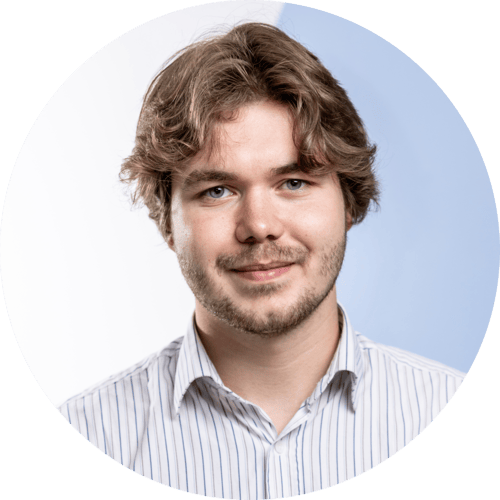
\includegraphics[width=2cm,clip]{images/EDY-pp-small.png}
}
\parbox{\dimexpr\linewidth-2.2cm\relax}{
\begin{tabularx}{\linewidth}{L r} \\
  \textbf{\Large \name} & \href{mailto:\emaila}{\raisebox{0.0\height}{\footnotesize \faEnvelope}\ {\emaila}} \\
  {\course} & \href{https://www.linkedin.com/in/antoine-edy/}{\footnotesize \faLinkedin}\ \ \href{https://scholar.google.com/citations?user=6cS484AAAAAJ}{\footnotesize \faGraduationCap}\ \ \href{https://github.com/antoineedy}{\footnotesize \faGithub}\ \ \href{https://huggingface.co/antoineedy}{\raisebox{-0.2\height}{
\includegraphics[height=0.9em]{images/logo-hf.jpeg}}}\ \ \href{https://x.com/antoine_edy}{\raisebox{-0.2\height}{
\includegraphics[height=0.8em]{images/logo-twitter.png}}} \\
  & {\footnotesize \faMapMarker*\ Paris, France} \\
\end{tabularx}
}
\vspace{-3mm}

%-----------PUBLICATIONS-----------------
\section{\makebox[\linewidth][s]{\textbf{Publications}\hfill{\normalfont\footnotesize\textit{$^\star$\,denotes equal contribution}}}}
\resumeSubHeadingListStart

     \resumeProject
      {DAEDALUS: Bootstrapping Agent Memory from Self-Generated Tasks}
      {}
      {}{}
    \vspace{-6mm}
      \resumeItemListStart
        \item {\textbf{A. Edy$^\star$}, M. Conti$^\star$, V. Xing$^\star$, M-A. Allard, N. Benhamdane, G. Viaud}
        \item {Self-improving agents that build their own memory by practicing on self-generated tasks, without training tasks or oracle verifiers. On AppWorld, $\tau^2$-bench and AutomationBench, strongest method without training tasks and competitive with those that use them; memory banks transfer across model families.}
        \item {\textbf{Preprint} (2026), \href{https://arxiv.org/abs/2610.08048}{{\tiny\faLink}\ arXiv:2610.08048}}
    \resumeItemListEnd

    \resumeProject
      {ViDoRe V3: A Comprehensive Evaluation of RAG in Complex Real-World Scenarios}
      {}
      {}{}
    \vspace{-6mm}
      \resumeItemListStart
        \item {A. Loison$^\star$, Q. Macé$^\star$, \textbf{A. Edy$^\star$}, V. Xing, T. Balough, G. Moreira, B. Liu, M. Faysse et al.}
        \item {Multimodal RAG benchmark: 26,000 pages, 18,594 queries across 10 domains in 6 languages, 12,000h of human annotation. Work made in collaboration with NVIDIA; $\sim$500k dataset downloads/year on \href{https://huggingface.co/collections/vidore/vidore-benchmark-v3}{\raisebox{-0.1\height}{
\includegraphics[height=0.7em]{images/logo-hf.jpeg}}\ Hugging Face}.}
        \item {\textbf{ACL 2026 Main Conference} (Oral Presentation), \href{https://arxiv.org/abs/2601.08620}{{\tiny\faLink}\ arXiv:2601.08620}}
    \resumeItemListEnd

    \resumeProject
      {Analyzing Targeted Behaviors of Late Interaction Models}
      {}
      {}{}
      \vspace{-6mm}
      \resumeItemListStart
        \item {\textbf{A. Edy$^\star$}, M. Conti$^\star$, Q. Macé$^\star$}
        \item {Analysis of length bias in multi-vector scoring and MaxSim similarity distribution on NanoBEIR benchmark}
        \item {\textbf{ECIR 2026} Late Interaction Workshop (Poster), \href{https://arxiv.org/abs/2603.26259}{{\tiny\faLink}\ arXiv:2603.26259}}
    \resumeItemListEnd
  \resumeSubHeadingListEnd
\vspace{-4mm}


%-----------EXPERIENCE-----------------
\section{\textbf{Experience}}
  \resumeSubHeadingListStart
\resumeSubheading
 {Illuin Technology}{Paris, France}
{AI Research Scientist}{September 2024 - Present}
\vspace{-6mm}
\resumeItemListStart
\item {First author of DAEDALUS: designed a self-improving agent that builds its own memory from self-generated practice tasks for in-context learning on long-horizon tool-use tasks}
\item {Co-led the creation of ViDoRe V3, establishing the gold standard benchmark for multimodal document retrieval evaluation; contributor to the MTEB ecosystem}
\item {Conducted research on Multimodal Retrieval and late interaction dynamics (ColBERT/ColPali-like models)}
\item {Fine-tuned LLMs for tool calling in agentic RAG contexts; fine-tuned speech-to-text models (Whisper, NVIDIA Parakeet) for domain-specific industrial applications}
\item {Conducted 50+ technical interviews as part of the hiring process for Data Scientist positions}
\resumeItemListEnd
    
    \resumeSubheading
      {Centre for Vision, Speech and Signal Processing (University of Surrey)}{Guildford, United-Kingdom}
      {Research Intern}{2024}
      \vspace{-6mm}
      \resumeItemListStart
    \item {Studied zero-shot semantic segmentation using multimodal foundation models; improved ZegCLIP baseline with multi-scaling techniques and inner encoder layers}
    \item {Research led to Master's thesis: \textit{Exploring Zero-Shot Capabilities of Multimodal Foundation Models for Semantic Segmentation}, supervised by Prof. Muhammad Awais Rana and Dr. Srinivasa Rao Nandam \href{https://www.researchgate.net/publication/384687820}{{\tiny\faLink}\ ResearchGate}}
    \resumeItemListEnd

    \resumeSubheading
      {AI-vidence}{Palaiseau, France}
      {ML Research Intern}{2023}
      \vspace{-6mm}
      \resumeItemListStart
    \item {Developed a Python library for tabular model explainability and cluster analysis}
    \item {Presented at SpringTech Paris-Saclay 2023 at HEC Paris}
    \resumeItemListEnd
      
  \resumeSubHeadingListEnd
\vspace{-4mm}



%-----------EDUCATION-----------
\section{\textbf{Education}}
  \resumeSubHeadingListStart
    \resumeSubheading
      {University of Surrey}{Guildford, United-Kingdom}
      {Master of Science in Artificial Intelligence}{2023-2024}
      \vspace{-6mm}
      \resumeItemListStart
    \item {International Excellence Scholarship recipient. Graduated with Highest Honors}
    \item {NLP, CV, Audio Processing, Symbolic Knowledge Representation and Logical Reasoning, People-Centered AI}
    \item {Master's Thesis: \textit{Zero-shot and Few-shot Adaptation of Multimodal Foundation Models}}
    \resumeItemListEnd
    
    \resumeSubheading
      {École Centrale de Lyon}{Lyon, France}
      {General Engineering Program (Grande École)}{2021-2024}
      \vspace{-6mm}
      \resumeItemListStart
    \item {Specializations: Mathematics, Machine Learning, Probability Theory, Chaos and Fractals}
    \item {Project Leader: Unsupervised MCU Classification with Deep Learning for STMicroelectronics}
    \resumeItemListEnd
    
    \resumeSubheading
      {Collège Stanislas Paris VI}{Paris, France}
      {Classe Préparatoire, MPSI-MP}{2019-2021}
  \resumeSubHeadingListEnd
\vspace{-5mm}
\vspace{-4mm}



%-----------TALKS-----------------
\section{\textbf{Talks \& Blog Posts}}
\vspace{-0.4mm}
\resumeSubHeadingListStart
\resumePOR{}
    {\textbf{Multimodal Retrieval and ViDoRe V3}, Invited talk, Neurons \& Peppers (Datacraft, Paris)} % Event
    {2026} %Event Year
\vspace{-1mm}
\resumePOR{}
    {\textbf{Agentic Search Framework for ViDoRe V3} \href{https://huggingface.co/blog/antoineedy/vidore-v3-pipeline-framework-and-leaderboard}{{\tiny\faLink}\ Hugging Face blogpost}}
    {2026}
\vspace{-1mm}
\resumePOR{}
    {\textbf{Xplique: analysing different scales of interpretability} \href{https://www.ai-vidence.com/xplique-la-librairie-python-pour-expliquer-le-vision-par-ordinateur/}{{\tiny\faLink}\ AI-vidence blogpost}}
    {2023}
\resumeSubHeadingListEnd
\vspace{-2mm}


% %-----------OPEN SOURCE-----------------
% \section{\textbf{Open Source Contributions}}
% \vspace{-0.4mm}
% \resumeSubHeadingListStart
% \resumePOR{}
%     {Contributor to MTEB, colpali-engine, vidore-benchmark, 
% widgetti apps}
%     {}
% \vspace{-1mm}
% \resumePOR{}
%     {Developer of istacky, an open-source Python image-processing library \href{https://github.com/antoineedy/istacky}{{\tiny\faLink}\ GitHub}}
%     {}
% \resumeSubHeadingListEnd
% \vspace{-5mm}


%-----------Technical skills & Hobbies (two columns)-----------------
\begin{minipage}[t]{0.66\textwidth}
\section{\textbf{Technical Skills}}
\begin{itemize}[leftmargin=0in, label={}]
 \small{\item{
\textbf{ML Frameworks}{: PyTorch, Hugging Face (Transformers, PEFT, Accelerate),  W\&B, NVIDIA NeMo, OpenMMLab} \\
\textbf{Information Retrieval}{: SentenceTransformer, pylate, colpali-engine, MTEB, FAISS, (Fast)PLAID}, ElasticSearch \\
\textbf{Infra. and Ops.}{: Kubernetes, Docker, vLLM, SLURM, HTCondor, skypilot, GCP} \\
\textbf{Languages}{: French (Native), English (C1, TOEFL 623/677), Spanish (B1)} \\
}}
\end{itemize}
\end{minipage}
\hfill
\begin{minipage}[t]{0.32\textwidth}
\section{\textbf{Hobbies}}
  \begin{itemize}[leftmargin=10pt, noitemsep, topsep=0pt, partopsep=0pt, parsep=0pt]
    \small{
    \item {Competitive tennis, football, and any sport going (any day, any time)}
    \item {Chess, where my tactics and my blunders are evenly matched}
    \item {Cinema, literature, hip-hop music}
    \item {Digital graphic design and art culture}
  }
    \end{itemize}
\end{minipage}
%\vspace{-16pt}



%-------------------------------------------
\end{document}
